The \model models allow to run from whole world experiments to small scale regions. In order to do so, three pymedeas models are provided, which are organized in two nestings:
\begin{itemize}
    \item The main model is the full world model (nesting level 0). This model repressents the full agreggated world system. This model is also called \modelsub{w}.
    \item The first nested model (nesting level 1) corresponds to a regional model, this model repressents a region of the world model. This model is also called \modelsub{rg}.
    \item The second nested model (nesting level 2) corresponds to a subregional model, this model repressents a subregion of the region used in the regional model.  This model is also called \modelsub{srg}.
\end{itemize}

\begin{figure}[H]
    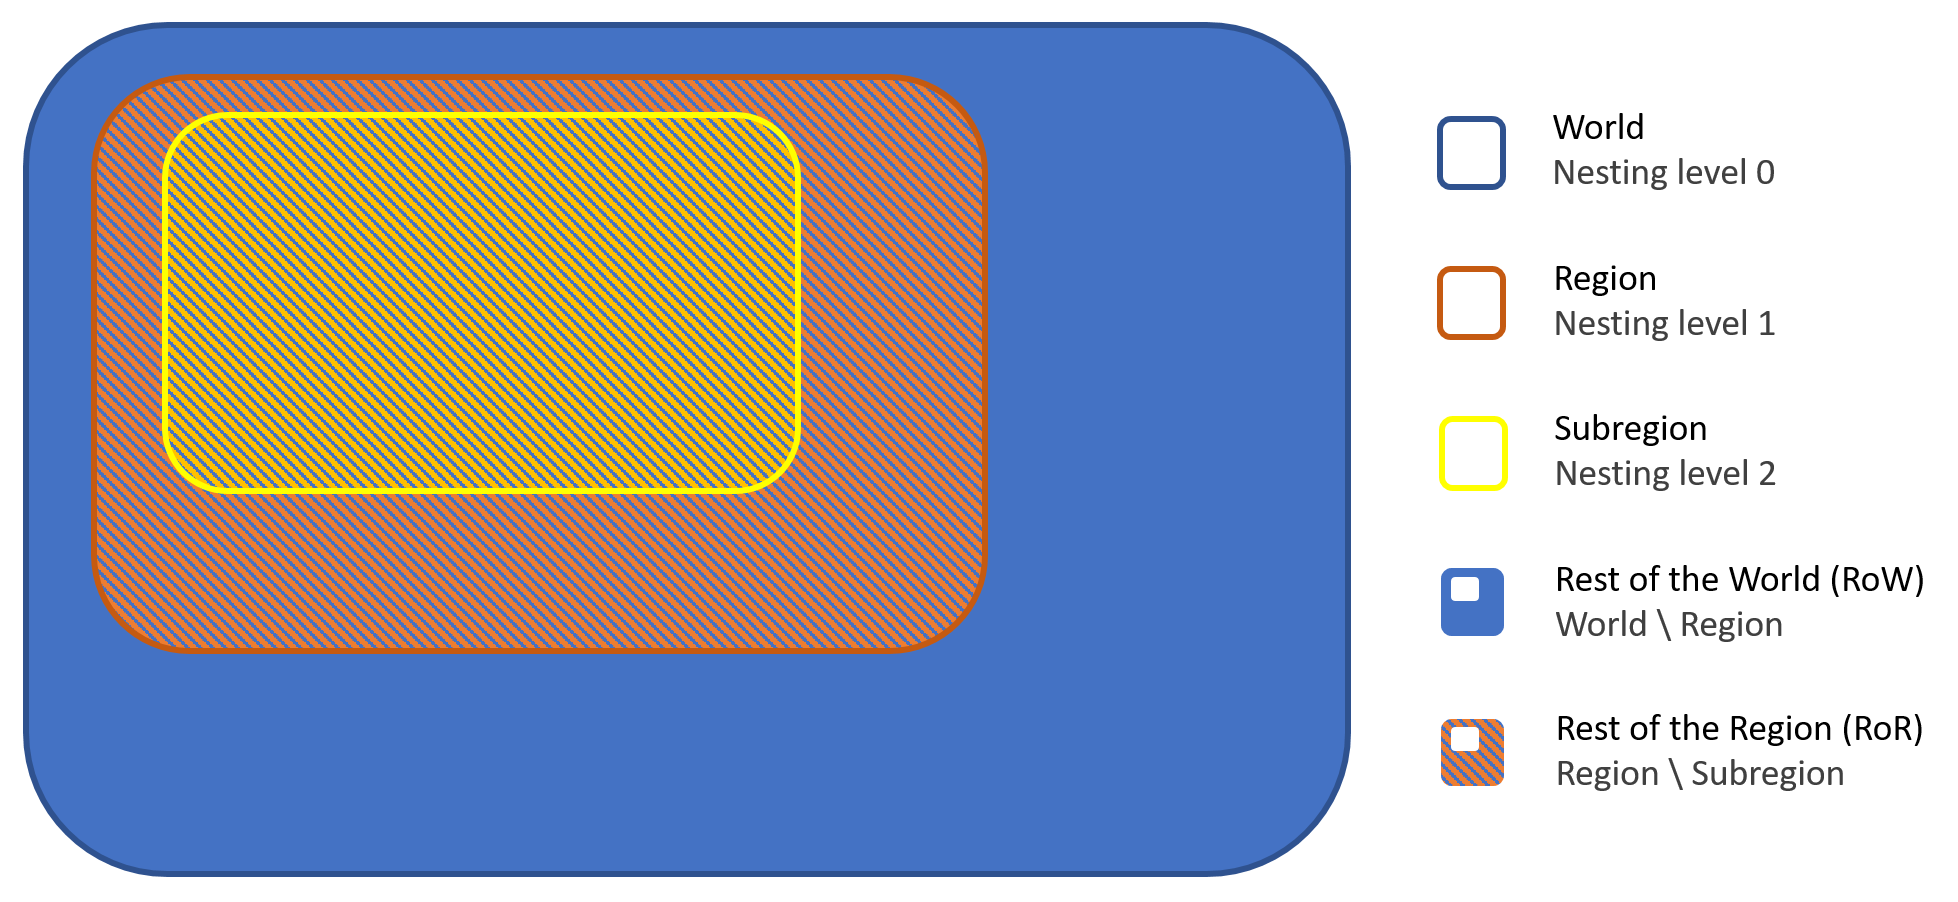
\includegraphics[width=\textwidth]{figures/nesting.png}
    \caption{Nesting of \model models}
    \label{fig:nesting}
\end{figure}

In the nested models we commonly refer to the complementary part of the region as rest of the world (RoW) or rest of the region (RoR). Therefore, Row repressents all the world except Region, and RoR repressents all the Region except Subregion, see the Figure \ref{fig:nesting}.

In order to run a nested model the upper... \note{Add runing nested models information}

